\chapter{GATE LEVEL SIMULATION}
\label{chap:gate_intro.tex}

In a typical VLSI design flow, the first step is creating an RTL level model of the design and writing the behavioral test bench for functional verification of this model. Once the functional RTL verification is completed, the next stage is design synthesis. During synthesis RTL is turned into a design implementation in terms of logic gates. Synthesis is mostly an automated process using a “{\it synthesizer}” tool that converts RTL-level design source code into gate-level netlist file.

 The netlist out of synthesis tool is then fed into layout tool which produces the layout of the design. During this process modifications are done on netlist but it remains functionally equal to its corresponding RTL. Netlist written by layout tool after layout has been done is called a post layout netlist.~\figurename{~\ref{fig:gatesim.eps}} shows where Gatesim comes in design flow.

%\figurename{} 
\begin{figure}[H]
\centering
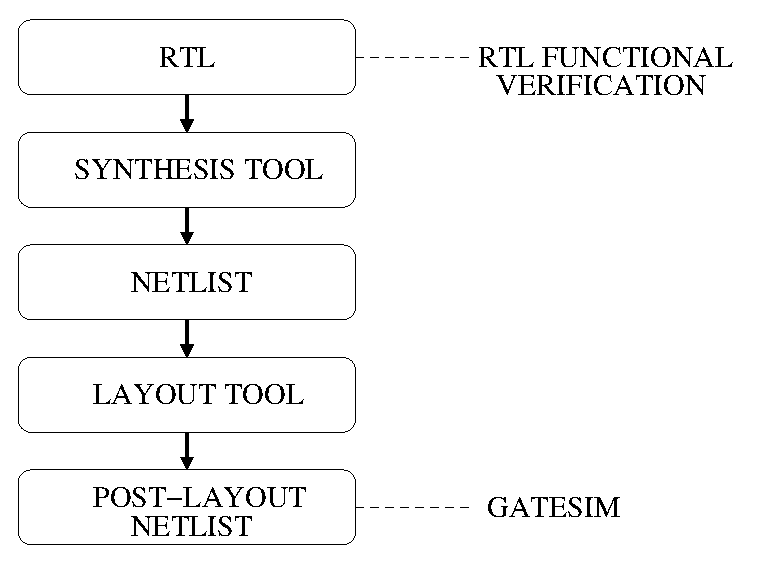
\includegraphics[width=3.5in]{./figures/gatesim.eps}
\caption{Design Flow}
\label{fig:gatesim.eps}
\end{figure}
Gate Level Simulation or Gatesim focuses on verifying the post layout netlist of a module. Originally developed for verifying the functional correctness of chip netlist when formal tool were not available; Gatesims are currently used to complement and cover gaps left by formal flow. 


\section {NEED FOR GATESIM}
Gatesims are generally used for verifying the following. 
\begin{itemize}
	\item[-]To check if power-up, reset operation and initialization of the design are proper.
	\item[-]The RTL written is synthesizable.
	\item[-]DFT structures that are absent in RTL and are added during or after synthesis, they are not checked by simulation.
	\item[-]The netlist passes all the critical test scenarios.
	\item[-]Any un-initialized outputs.
	\item[-]Low-power structures that are absent in RTL and added later during synthesis.
	\item[-]Can be used to study the activity factor for power estimation.
	\item[-]X's in RTL simulation can be pessimistic or optimistic. Any issues caused due to this can be found by Gatesims.
	\item[-]STA does not analyze asynchronous interfaces.
\end{itemize}

Finally, Gatesim is a great confidence-booster in ensuring the high quality of the netlist. It lowers the risk of finding late design issues.




\section{LIMITATIONS OF LEC AND STA}

Gatesims are done after RTL code is simulated and synthesized into a gate level netlist. Other importance verification steps like Logic equivalence check (LEC) and Static Timing Analysis are also done after RTL synthesis. 

\emph {\bf LEC}: Logic Equivalence Checking (LEC) is a formal verification tool that compares a reference design against a derived design to prove equivalence or to report differences.  LEC does not require test patterns. Instead, LEC uses Boolean arithmetic techniques to prove equivalence between two design netlists. Although LEC uses sophisticated formal algorithms to identify, map, and compare nodes in the netlists, the complexity is hidden from the user [ieee].

\emph {\bf STA}: Static Timing analysis does a input-independent timing analysis of the gate level netlist. It locates the worst-case delay of the circuit over all possible conditions. There are huge numbers of logic paths inside a chip of complex design. The advantage of STA is that it performs timing analysis on all possible paths (whether they are real or potential false paths). 



These formal static verification techniques are much faster and evolved than simulation based methods. However these verification methodologies, in spite of advancements in tools, do not cover all aspects. Gatesim helps in filling up the gaps left by these methods. 

Some of the issues with LEC can be solved by Gatesims. The following are some issues encountered during real SoC design project execution: 

\begin{itemize}
	\item Limitation of Static Equivalence Checking tools to catch X-propagation issues.
	\item Two-state methodologies can miss RTl-versus-netlist simulation and RTL-versus-RTL simulation differences.
	\item Incorrect mapping issues due to naming at sub-block level which can result in false pass. This will not be reported at the sub-block level LEC, but Gatesims can flag such incorrect connectivity.
\end{itemize}
Some of the STA limitations that can be covered by Gatesims are:
\begin{itemize}
	\item \emph{\bf X-handling:} STA deals only with logic domain of logic-0 and logic-1. An X in the design cause undetermined values to propagate through the design. This cannot be checked with STA
	\item \emph{\bf Interfaces between analog and digital blocks:} STA does not deal with analog blocks. And hence cannot verify connectivity between digital and analog blocks where as Gatesims can.
	\item \emph{\bf Reset sequence:} Verifying that all flip-flops resets into their required logical value. STA cannot check this as certain declarations such as initial values on signal are not synthesizable and are verified only during simulation.
	\item \emph{\bf Asynchronous clock-domain crossings:} STA does not check if the correct clock synchronizers are being used.
\end{itemize}








\section{ISSUES CAUGHT BY GATESIM}
%\section{DYNAMICALLY RECONFIGURABLE \\DATA-PATH}
The following are design issues missed initially but caught by gatesims:
\begin{enumerate}
		
	\item \emph{\bf X Squashing}

	X-Squashing is a term used when X-es get squashed in a simulation and don't propagate anymore through the logic. In an example there was an X-Squashing issue in behavioral RTL which led to a valid value being present in one of the RTL outputs during simulations, where as in gates X wasn't squashed and it propagated to the corresponding output resulting in a simulation mismatch between RTL and gates.

	\item \emph{\bf Reset X problem}

	Some of the un-initialized flops resulting in X issues were easily found during GLS.  After identifying such scenarios appropriate forces were added as part of Gate simulation flow.

	\item \emph{\bf Wrong connectivity during block level mapping}

	During integration, sub-blocks at top level may get connected incorrectly due to naming issues at the sub block level. Sub-block level LEC would not catch this issue, whereas gatesim flags the wrong connectivity.
\end{enumerate}







\section{ISSUES OF GATESIM}
At system level, Gatesim is one of the most challenging verification domains. This is because with higher design complexity, limitations of gatesim become more prominent. Main difficulties associated with gate level simulation are:
\begin{itemize}


\item[-] Larger turn-around time (run, debug cycle).
\item[-] Limitation on size of netlist that can be verified through gatesim. This is an indirect cause due to larger build times and run times.
\item[-] Debugging the netlist simulation is challenging.
\item[-] Huge compute resource utilization. 

\end{itemize}
